% 编译方式：XeLaTeX，连续编译两次。
% 将本文件与 figures 文件夹一起上传 Overleaf，并选择 XeLaTeX。
\documentclass[UTF8,a4paper,zihao=-4,fontset=fandol]{ctexart}
\usepackage[margin=2.5cm]{geometry}
\usepackage{amsmath,amssymb,booktabs,tabularx,array,graphicx}
\usepackage{caption,float,placeins}
\usepackage[hidelinks]{hyperref}
\usepackage{fancyhdr}
\graphicspath{{figures/}}
\captionsetup{font=small,labelsep=quad}
\setlength{\parindent}{2em}
\setlength{\parskip}{0.25em}
\renewcommand{\arraystretch}{1.2}
\pagestyle{fancy}
\fancyhf{}
\fancyhead[C]{\small 基于深度神经网络的猫狗图像分类}
\fancyfoot[C]{\thepage}
\setlength{\headheight}{15pt}
\newcolumntype{Y}{>{\raggedright\arraybackslash}X}
% 请在提交前填写以下信息。
\newcommand{\studentname}{\underline{\hspace{3cm}}}
\newcommand{\studentid}{\underline{\hspace{3cm}}}
\newcommand{\studentclass}{\underline{\hspace{3cm}}}

\begin{document}
\begin{titlepage}
  \centering
  \vspace*{2cm}
  {\zihao{2}\heiti 自然语言处理课程实验报告\par}
  \vspace{1.2cm}
  {\zihao{1}\heiti 基于深度神经网络的\par 猫狗图像分类\par}
  \vspace{0.8cm}
  {\zihao{3} DNN、CNN 与 RNN 的设计及正则化分析\par}
  \vspace{2cm}
  {\zihao{4}\renewcommand{\arraystretch}{1.8}
  \begin{tabular}{rl}
    作业名称：&作业一\\
    姓\qquad 名：&\studentname\\
    学\qquad 号：&\studentid\\
    班\qquad 级：&\studentclass\\
  \end{tabular}\par}
  \vfill
  {\large 实验框架：PyTorch\par}
  \vspace{1cm}
\end{titlepage}

\begin{abstract}
为掌握深度神经网络的基本结构及其在深度学习框架中的实现方法，本实验根据课程作业要求，在给定猫狗图像数据集上设计并实现了深度前馈网络（DNN）、卷积神经网络（CNN）和循环神经网络（RNN）。三个模型分别采用分块全连接混合、残差卷积和行列双向 GRU 进行特征提取。在统一的数据划分、输入尺寸和训练轮数下，通过增强权重衰减及 Dropout 开展正则化对照实验，并结合逐类准确率、混淆矩阵和损失曲线分析模型表现。正则化后，DNN、CNN、RNN 的最佳普通验证准确率分别为 69.2\%、83.6\% 和 70.4\%；CNN 的猫类、狗类准确率分别为 82.4\% 和 84.8\%，取得最好的综合表现。曲线表明，DNN 后期过拟合仍较明显，CNN 后期存在泛化差距与波动，RNN 的验证损失则较早进入平台期。实验进一步说明，最高验证准确率与最低验证损失可以对应不同轮次；以分类正确率为目标时，可以优先按验证准确率选取模型，但应同时报告过拟合迹象，并区分验证集选择结果与独立测试集上的泛化结论。
\end{abstract}
\noindent\textbf{关键词：}猫狗分类；深度神经网络；卷积神经网络；循环神经网络；正则化；过拟合
\newpage
\tableofcontents
\newpage

\section{实验目的与任务要求}
课程作业要求使用一种深度学习框架，分别实现基于 DNN、CNN 和 RNN 的猫狗图像分类模型，具体网络结构可以自行设计；由于两类样本数量一致，需报告各类别的准确率，并提交代码与实验报告。本实验采用 PyTorch，围绕数据处理、网络设计、参数优化、模型选择和结果分析构建完整实验流程。

猫狗分类属于二分类任务。给定输入图像 $x$，模型输出两个类别的得分，再以得分较大的类别作为预测结果。本实验的重点是比较不同结构对图像特征的表达能力，并研究在有限样本条件下，增强正则化是否能够改善模型的验证表现。

作业将 \texttt{val} 中的 500 张图像用于模型测试。在实际训练流程中，这部分数据还用于逐轮选择权重和比较配置，因此本文将其准确称为\textbf{验证集}。文中结果不等同于未参与模型选择的独立测试集成绩。

\section{数据集与预处理}
数据来自作业提供的猫狗图像数据集。按作业说明，原始图像来源于 Kaggle 猫狗分类数据。实验保持给定的训练与验证划分，不引入外部图像或预训练权重。

\begin{table}[htbp]
\centering
\caption{数据集规模}
\begin{tabular}{lrrr}
\toprule
数据划分 & 猫 & 狗 & 总计\\
\midrule
训练集 & 1,000 & 1,000 & 2,000\\
验证集 & 250 & 250 & 500\\
\bottomrule
\end{tabular}
\end{table}

首先校正图像的 EXIF 方向，将图像统一转换为 RGB 格式，再通过双线性插值缩放到 $64\times64$。将像素从 $[0,255]$ 映射到 $[-1,1]$，得到输入张量 $x\in\mathbb{R}^{B\times3\times64\times64}$，其中 $B$ 为批量大小。训练阶段以 $0.5$ 的概率水平翻转图像；验证阶段采用确定性预处理，不加入随机增强。

水平翻转在不改变类别的条件下增加了朝向变化，但没有产生新的主体、背景或拍摄条件，其增强能力有限。统一到较低分辨率可以降低计算成本，同时也可能损失部分细节；这一限制在三个模型中保持一致。

\section{网络结构设计}
\subsection{DNN：基于图像分块的全连接混合网络}
\subsubsection{基本原理}
深度前馈网络通过多层线性映射和非线性激活建立输入与类别之间的关系。单层变换可写为
\begin{equation}
 h^{(l+1)}=\phi\bigl(W^{(l)}h^{(l)}+b^{(l)}\bigr),
\end{equation}
其中 $\phi$ 为非线性激活函数。本实验的 DNN 使用图像分块与全连接混合结构，不包含卷积层或循环层。

\subsubsection{具体实现}
将 $64\times64$ 图像划分为 $8\times8$ 大小的不重叠图像块，共得到 $64$ 个块。每块展开为 $3\times8\times8=192$ 维向量，通过共享线性层映射到 128 维，得到 $T\in\mathbb{R}^{B\times64\times128}$。

随后堆叠四个残差混合模块。每个模块依次进行图像块维度混合和通道维度混合。记 $\mathrm{LN}$ 为对特征通道的 LayerNorm，省略批维，则计算可表示为
\begin{align}
 U &= T+\left[\mathrm{MLP}_{\mathrm{token}}\bigl(\mathrm{LN}(T)^{\mathsf T}\bigr)\right]^{\mathsf T},\\
 V &= U+\mathrm{MLP}_{\mathrm{channel}}\bigl(\mathrm{LN}(U)\bigr).
\end{align}
其中图像块混合 MLP 的维度为 $64\rightarrow64\rightarrow64$，通道混合 MLP 的维度为 $128\rightarrow256\rightarrow128$，均使用 GELU 激活。图像块混合在激活后使用 Dropout；通道混合在激活后及第二个线性层后使用 Dropout，概率均为 $0.3$。残差相加保持张量尺寸不变。

四个模块之后进行 LayerNorm，再对 64 个块取平均，形成 128 维图像表示，经过概率为 $0.4$ 的 Dropout 和 $128\rightarrow2$ 线性层完成分类。

\begin{table}[htbp]
\centering\small
\caption{DNN 各阶段输出尺寸（省略批量维度）}
\begin{tabularx}{\textwidth}{lYl}
\toprule
阶段 & 主要操作 & 输出尺寸\\
\midrule
图像分块 & 64 个 $8\times8$ RGB 块并展开 & $64\times192$\\
块特征映射 & 共享线性层 $192\rightarrow128$ & $64\times128$\\
混合模块 $\times4$ & 图像块混合、通道混合、残差相加 & $64\times128$\\
特征汇总 & LayerNorm、块维度平均 & $128$\\
分类头 & Dropout、线性层 & $2$\\
\bottomrule
\end{tabularx}
\end{table}

该网络共有 324,226 个参数。分块映射共享局部输入的处理方式，混合模块则建立块之间的联系；但其空间约束与卷积不同，对位置相关性及训练样本数量可能更敏感。

\subsection{CNN：残差卷积网络}
\subsubsection{基本原理}
卷积网络利用局部连接和位置间的权重共享提取图像特征。浅层卷积可以学习局部纹理与边缘，随着层数增加及空间下采样，网络可以组合更大范围的信息。本实验采用残差连接，将卷积分支与输入投影相加，使网络能够在已有表示上学习增量特征。

\subsubsection{具体实现}
网络包含三个残差卷积块，输出通道依次为 32、64、128。每块的主分支由两个不带偏置的 $3\times3$ 卷积构成，步长为 1、填充为 1。每个卷积后接分为 8 组的 GroupNorm，第一个归一化之后接 ReLU。跳跃分支使用 $1\times1$ 卷积匹配通道。若记主分支为 $F$、投影分支为 $P$，则块输出为
\begin{equation}
 y=\mathrm{MaxPool}_{2\times2}\bigl(\mathrm{ReLU}(F(x)+P(x))\bigr).
\end{equation}
三个块之后的特征图为 $128\times8\times8$，经自适应平均池化变为 $128\times2\times2$，展开为 512 维。分类头依次执行 $512\rightarrow128$ 线性映射、ReLU、概率为 $0.35$ 的 Dropout 和 $128\rightarrow2$ 线性映射。

\begin{table}[htbp]
\centering\small
\caption{CNN 各阶段输出尺寸（省略批量维度）}
\begin{tabular}{lll}
\toprule
阶段 & 通道或映射 & 输出尺寸\\
\midrule
输入图像 & RGB & $3\times64\times64$\\
残差卷积块 1 & $3\rightarrow32$ & $32\times32\times32$\\
残差卷积块 2 & $32\rightarrow64$ & $64\times16\times16$\\
残差卷积块 3 & $64\rightarrow128$ & $128\times8\times8$\\
自适应平均池化 & 输出空间尺寸 $2\times2$ & $128\times2\times2$\\
分类头 & $512\rightarrow128\rightarrow2$ & $2$\\
\bottomrule
\end{tabular}
\end{table}

CNN 共包含 363,714 个参数。其局部空间建模方式与图像分类任务相匹配。GroupNorm 在样本内部按通道分组计算统计量，不依赖批量维度的统计估计。

\subsection{RNN：行列双向 GRU 网络}
\subsubsection{基本原理}
循环神经网络通过递归更新隐藏状态处理序列。门控循环单元 GRU 使用重置门和更新门控制历史信息与当前输入的组合。以单方向 GRU 为例，与本项目所用 PyTorch GRU 对应的更新形式为
\begin{align}
 r_t &= \sigma(W_{ir}x_t+b_{ir}+W_{hr}h_{t-1}+b_{hr}),\\
 z_t &= \sigma(W_{iz}x_t+b_{iz}+W_{hz}h_{t-1}+b_{hz}),\\
 n_t &= \tanh\bigl(W_{in}x_t+b_{in}+r_t\odot(W_{hn}h_{t-1}+b_{hn})\bigr),\\
 h_t &= (1-z_t)\odot n_t+z_t\odot h_{t-1},
\end{align}
其中 $r_t$、$z_t$ 分别为重置门和更新门，$\odot$ 为逐元素乘法。双向 GRU 从两个相反方向读取序列，并拼接两个方向的隐藏状态。

\subsubsection{图像序列化与分类}
本实验分别按行、列组织图像。行序列的每个时间步包含一整行 RGB 像素，维度为 $3\times64=192$，序列长度为 64；列序列同理。两路分别使用独立的 $192\rightarrow64$ 线性层、LayerNorm 和 GELU，然后输入各自的单层双向 GRU，单方向隐藏维度为 64。因此，每路输出为 $64\times128$。

对每路的全部时间步取平均，再将行、列特征拼接：
\begin{equation}
 g=\left[\frac{1}{64}\sum_{t=1}^{64}h_t^{\mathrm{row}}\ ;\ 
          \frac{1}{64}\sum_{t=1}^{64}h_t^{\mathrm{col}}\right]\in\mathbb{R}^{256}.
\end{equation}
最后经过 LayerNorm、概率为 $0.4$ 的 Dropout 和 $256\rightarrow2$ 线性层输出类别得分。Dropout 位于分类头，不施加在 GRU 循环连接上。

\begin{table}[htbp]
\centering\small
\caption{RNN 各阶段输出尺寸（省略批量维度）}
\begin{tabularx}{\textwidth}{lYl}
\toprule
阶段 & 主要操作 & 输出尺寸\\
\midrule
行、列序列化 & 每行或每列展开为 RGB 向量 & 每路 $64\times192$\\
输入投影 & 线性层、LayerNorm、GELU & 每路 $64\times64$\\
双向 GRU & 每方向隐藏维度 64 & 每路 $64\times128$\\
时间平均与拼接 & 两路平均特征拼接 & $256$\\
分类头 & LayerNorm、Dropout、线性层 & $2$\\
\bottomrule
\end{tabularx}
\end{table}

该网络共有 125,826 个参数。行列两路提供互补的扫描方向，但二维局部关系需要通过序列表示间接表达，与 CNN 的局部卷积具有不同的结构偏好。
\FloatBarrier

\section{训练方法与评价指标}
\subsection{损失函数与优化设置}
三个模型均输出两个未归一化得分，训练时直接传入交叉熵损失，无须在网络末端额外添加 Softmax 层。设 $p_{i,y_i}$ 为第 $i$ 个样本经 Softmax 后分配给真实类别的概率，则
\begin{equation}
 \mathcal{L}_{\mathrm{CE}}=-\frac{1}{N}\sum_{i=1}^{N}\log p_{i,y_i}.
\end{equation}
使用 AdamW 优化器，从随机初始化训练 30 轮，不启用早停。每个模型训练前重置随机种子为 43。公共参数见表\ref{tab:common}。

\begin{table}[htbp]
\centering\caption{公共训练设置}\label{tab:common}
\begin{tabular}{ll}
\toprule
项目 & 设置\\
\midrule
框架与计算设备 & PyTorch，CUDA\\
输入尺寸 & $3\times64\times64$\\
优化器 & AdamW\\
学习率 & 固定 $3\times10^{-4}$\\
批量大小 & 32\\
训练轮数与随机种子 & 30 轮，种子 43\\
数据增强 & 训练时以 0.5 概率水平翻转\\
验证方式 & 原图推理，评估模式，不更新参数\\
\bottomrule
\end{tabular}
\end{table}

\subsection{正则化对照设置}
针对原实验中的训练与验证差距，本次保留网络结构、数据划分及上述公共设置，仅增强权重衰减和 Dropout。具体参数见表\ref{tab:reg}。Dropout 在训练阶段随机置零部分激活，验证阶段关闭；AdamW 通过权重衰减约束参数增长。损失日志记录数据上的交叉熵，没有额外加上一个权重衰减损失项。

\begin{table}[htbp]
\centering\small\caption{正则化参数调整}\label{tab:reg}
\begin{tabularx}{\textwidth}{lccY}
\toprule
模型 & 原权重衰减 & 新权重衰减 & Dropout 调整\\
\midrule
DNN & $10^{-4}$ & $10^{-3}$ & 混合模块 $0.2\rightarrow0.3$；分类头 $0.3\rightarrow0.4$\\
CNN & $10^{-4}$ & $5\times10^{-4}$ & 分类头 $0.3\rightarrow0.35$\\
RNN & $10^{-4}$ & $10^{-3}$ & 分类头 $0.3\rightarrow0.4$\\
\bottomrule
\end{tabularx}
\end{table}

\subsection{评价指标与最佳权重选择}
依据作业要求，分别计算猫、狗两类的准确率。本文的类别准确率定义为真实属于该类的样本中被正确识别的比例，等价于该类召回率：
\begin{equation}
 A_c=\frac{\sum_i\mathbf{1}(y_i=c\land\hat y_i=c)}{\sum_i\mathbf{1}(y_i=c)}.
\end{equation}
同时计算总体准确率 $A=\frac{1}{N}\sum_i\mathbf{1}(\hat y_i=y_i)$。由于验证集两类各 250 张，$A=(A_{\mathrm{cat}}+A_{\mathrm{dog}})/2$。此外报告验证交叉熵和混淆矩阵，以补充分类结果与错误分布信息。

每轮结束后评估验证集，优先保存总体验证准确率最高的权重；准确率相同时，选择验证损失较低的轮次。该规则与本实验以分类正确率为主要目标的设定一致。最后一轮权重另行保存，不能自动视为最佳模型。

\section{实验结果}
\subsection{正则化后的分类表现}
表\ref{tab:result}给出正则化后各模型的最佳轮次与指标。三个模型的结果均采用普通原图推理。现有评估脚本对 CNN 可执行原图与水平翻转图的得分平均，该结果不混入本表。

\begin{table}[htbp]
\centering\small
\caption{正则化后最佳模型的验证结果}\label{tab:result}
\begin{tabular}{lrrrrr}
\toprule
模型 & 最佳轮次 & 猫类准确率 & 狗类准确率 & 总体准确率 & 验证损失\\
\midrule
DNN & 11 & 84.0\% & 54.4\% & 69.2\% & 0.6568\\
CNN & 23 & 82.4\% & 84.8\% & \textbf{83.6\%} & 0.4174\\
RNN & 28 & 70.0\% & 70.8\% & 70.4\% & 0.6063\\
\bottomrule
\end{tabular}
\end{table}

混淆矩阵以行为真实类别、列为预测类别，类别顺序均为猫、狗：
\begin{equation}
 C_{\mathrm{DNN}}=\begin{pmatrix}210&40\\114&136\end{pmatrix},\quad
 C_{\mathrm{CNN}}=\begin{pmatrix}206&44\\38&212\end{pmatrix},\quad
 C_{\mathrm{RNN}}=\begin{pmatrix}175&75\\73&177\end{pmatrix}.
\end{equation}
CNN 的总体准确率最高，两类表现也较均衡。DNN 两类准确率相差 29.6 个百分点，114 张狗被预测成猫，而猫被预测成狗的数量为 40。这表明总体准确率不能完全反映其类别间表现差异。由于类别样本数相同，该差异不能归因于数量不平衡；具体原因仍需逐张检查错误样本。

\subsection{与原配置比较}
表\ref{tab:comparison}使用相同验证方式，比较原配置与正则化配置各自选出的最佳权重。
\begin{table}[htbp]
\centering\small
\caption{正则化前后的最佳验证结果比较}\label{tab:comparison}
\begin{tabular}{lrrrr}
\toprule
模型 & 原准确率 & 新准确率 & 变化（百分点） & 验证损失（原 $\rightarrow$ 新）\\
\midrule
DNN & 69.4\% & 69.2\% & $-0.2$ & $0.7434\rightarrow0.6568$\\
CNN & 83.0\% & 83.6\% & $+0.6$ & $0.4545\rightarrow0.4174$\\
RNN & 70.0\% & 70.4\% & $+0.4$ & $0.6078\rightarrow0.6063$\\
\bottomrule
\end{tabular}
\end{table}

按事先确定的准确率优先标准，CNN、RNN 新配置在本次验证中更好；DNN 的准确率略降，不能因验证损失降低而认定其分类效果已经提升。若在已有两组实验中选择每类最高验证准确率模型，应选择原配置 DNN，以及正则化后的 CNN、RNN；本文的主体结果仍完整报告本轮正则化实验，避免只保留有利结果。

500 张验证图像中，0.2 个百分点对应 1 张图像。CNN、RNN 的提升分别相当于净多识别正确 3 张和 2 张，DNN 则少 1 张。本次只有一个随机种子，尚不能认定这些差异具有统计显著性或稳定可重复性。同时调整了权重衰减和 Dropout，也无法区分两者各自的贡献。
\FloatBarrier

\section{损失曲线与过拟合分析}
\subsection{曲线判读原则}
训练损失持续下降，而验证损失不再改善甚至升高，同时验证准确率停滞或下降，是过拟合的重要迹象。但不能仅凭训练损失低于验证损失判断严重过拟合：本实验的训练指标在开启 Dropout、随机翻转及逐批更新参数时累积；验证指标来自每轮结束后的固定模型，且关闭 Dropout。两者测量条件不同，早期验证损失低于训练损失并不反常。

以下曲线的蓝线为训练交叉熵，橙线为验证交叉熵，绿色虚线标记最低验证损失轮次，紫色点线标记按既定规则选择的最佳准确率轮次。各模型关键轮次汇总见表\ref{tab:epochs}。

\begin{table}[htbp]
\centering\small
\caption{正则化实验关键轮次的指标}\label{tab:epochs}
\begin{tabular}{llrrrr}
\toprule
模型 & 观察点 & 轮次 & 训练损失 & 验证损失 & 验证准确率\\
\midrule
DNN & 最低验证损失 & 7 & 0.5791 & 0.6161 & 68.2\%\\
& 最佳验证准确率 & 11 & 0.5236 & 0.6568 & 69.2\%\\
& 最后一轮 & 30 & 0.3133 & 0.8368 & 64.6\%\\
\midrule
CNN & 最低验证损失 & 19 & 0.3409 & 0.4149 & 81.8\%\\
& 最佳准确率并以损失择优 & 23 & 0.2815 & 0.4174 & 83.6\%\\
& 最后一轮 & 30 & 0.1843 & 0.4359 & 83.6\%\\
\midrule
RNN & 最低验证损失 & 7 & 0.6034 & 0.5958 & 67.0\%\\
& 最佳验证准确率 & 28 & 0.4629 & 0.6063 & 70.4\%\\
& 最后一轮 & 30 & 0.4626 & 0.6126 & 67.6\%\\
\bottomrule
\end{tabular}
\end{table}

\subsection{DNN 的后期过拟合}
\begin{figure}[htbp]
\centering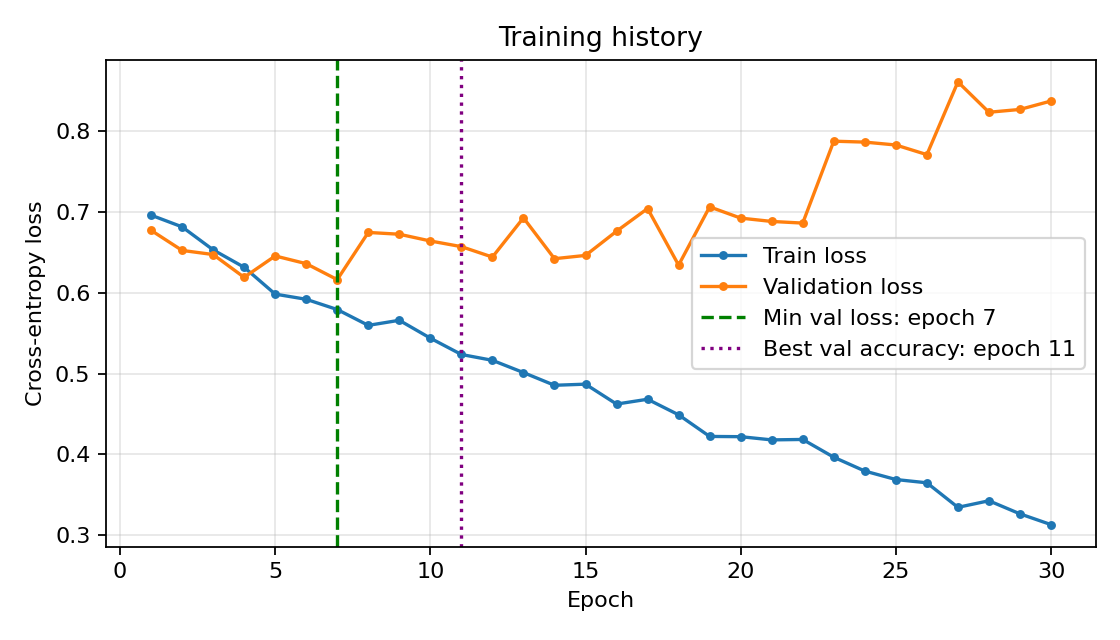
\includegraphics[width=0.9\textwidth]{dnn_loss.png}
\caption{DNN 正则化后的训练与验证损失}\label{fig:dnn}
\end{figure}
图\ref{fig:dnn}中，前几轮训练与验证损失总体同步下降。第 7 轮验证损失达到最低值 0.6161，之后虽然有波动和回落，但没有再次创新低；训练损失则继续下降，第 23 轮以后两条曲线的分离更加明显。第 30 轮训练准确率达到 86.15\%，验证准确率却降到 64.6\%，支持后期明显过拟合的判断。

第 11 轮已经存在泛化差距，但其验证准确率仍比第 7 轮高 1.0 个百分点。因此，第 11 轮可以是准确率意义上的最佳模型，同时不是交叉熵意义上的最佳模型。原配置末轮验证损失为 1.0066，本次降至 0.8368，说明后期交叉熵恶化程度有所缓解；但本次末轮准确率低于原来的 67.0\%，最佳准确率也未提高，不能据此认定全面改善。
\FloatBarrier

\subsection{CNN 的后期差距与波动}
\begin{figure}[htbp]
\centering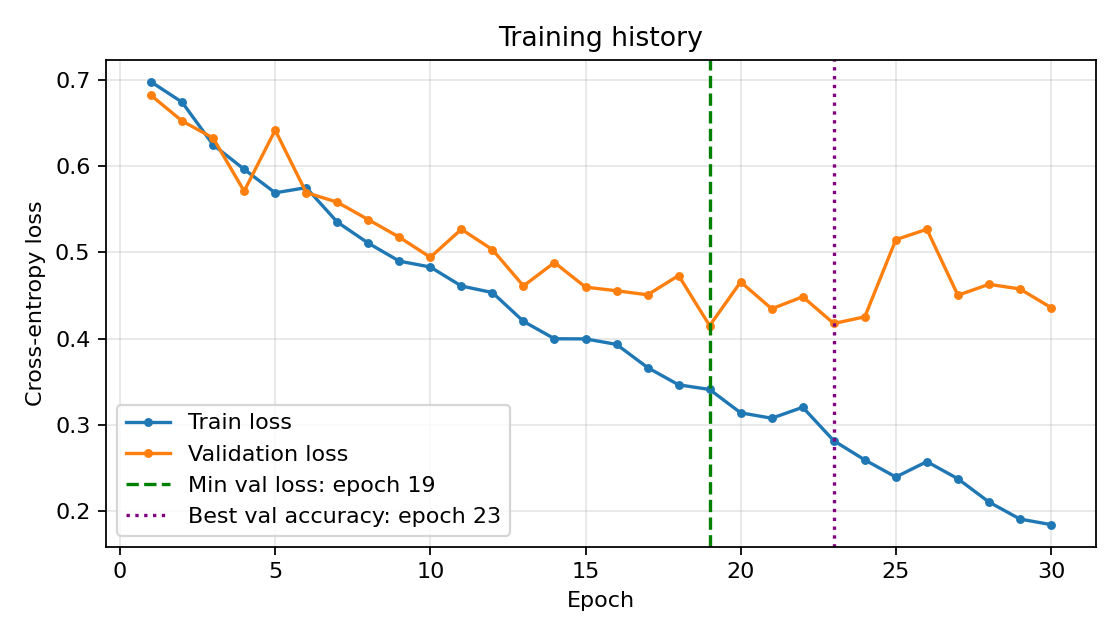
\includegraphics[width=0.9\textwidth]{cnn_loss.png}
\caption{CNN 正则化后的训练与验证损失}\label{fig:cnn}
\end{figure}
图\ref{fig:cnn}显示，CNN 在前 19 轮的验证损失总体下降，说明训练有效改善了验证表现。之后训练损失继续下降，验证损失却未创新低；第 25、26 轮升至约 0.51、0.53，随后又回落。因此后期存在过拟合迹象与波动，但不能描述为验证表现一直恶化。

第 23 轮比最低损失的第 19 轮净多识别正确 9 张图像，验证损失仅增加约 0.0025。对于准确率优先的任务，第 23 轮是合理选择。第 30 轮也达到 83.6\%，但损失为 0.4359，高于第 23 轮的 0.4174，因此程序仍保留第 23 轮权重。第 23 轮训练与验证准确率差为 5.55 个百分点，末轮扩大到 9.10 个百分点，需要结合测量条件理解。

与原配置相比，本次所选模型的准确率与损失均有改善；但最低验证损失仅从 0.4151 变为 0.4149，差异很小。更稳妥的结论是当前验证集表现小幅改善，后期过拟合仍然存在。
\FloatBarrier

\subsection{RNN 的验证损失平台期}
\begin{figure}[htbp]
\centering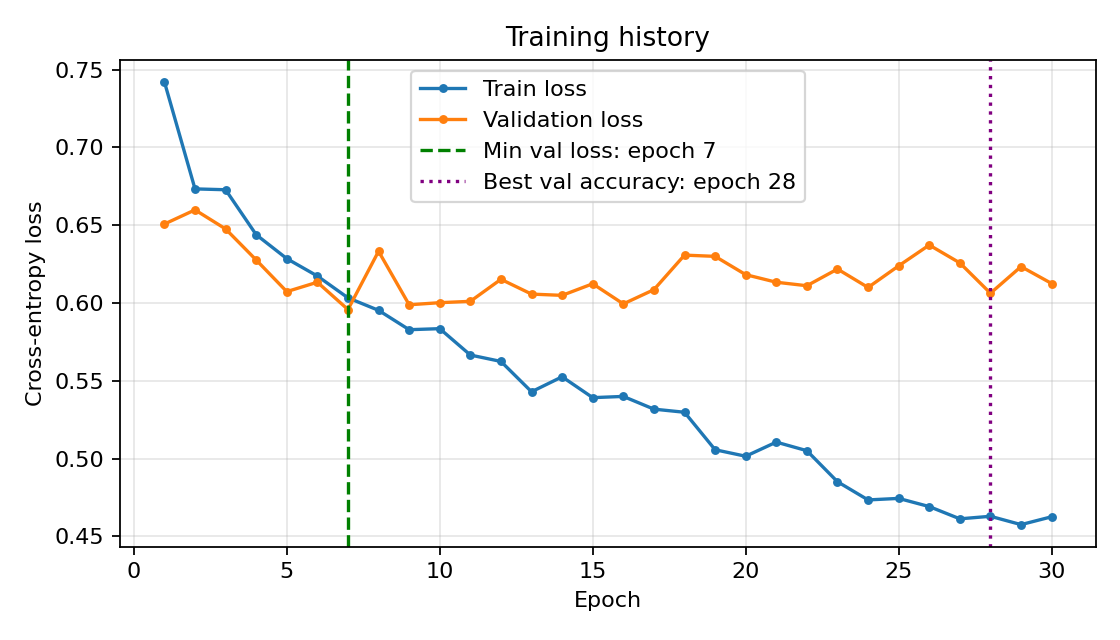
\includegraphics[width=0.9\textwidth]{rnn_loss.png}
\caption{RNN 正则化后的训练与验证损失}\label{fig:rnn}
\end{figure}
图\ref{fig:rnn}中，前 7 轮验证损失总体下降，之后大多在 0.60 至 0.64 附近波动，而训练损失继续降至约 0.46。后期收益主要体现在训练集，存在过拟合倾向，但验证损失没有像 DNN 那样大幅持续上升。

第 28 轮比第 7 轮的验证损失高约 0.0105，准确率却从 67.0\% 提高到 70.4\%，净多识别正确 17 张图像。仅按最低验证损失选第 7 轮，会牺牲本次观察到的分类准确率。末轮准确率又降至 67.6\%，说明最后一轮不等于最佳模型。原配置最低验证损失为 0.5932，本次为 0.5958，未见改善；最佳准确率的小幅提高不能解释为过拟合已经解决。
\FloatBarrier

\section{问题与思考}
\subsection{出现过拟合迹象后能否按最高验证准确率选模型}
对于以分类正确率为主要目标的任务，可以将验证准确率作为模型选择的首要指标，准确率相同时再比较验证损失。但应将结果表述为“当前验证集上、已评估轮次中准确率最佳的模型”，而不是已经证明泛化能力最强的模型。

准确率只关注预测类别是否正确，交叉熵还考虑模型为真实类别分配的概率。例如，真实为狗的图像，其狗类预测概率由 0.4 降为 0.01，两次均分类错误，因此准确率不变，但单样本交叉熵由约 0.916 增至 4.605。若模型同时纠正了其他若干图像，总准确率可能提高，平均损失却仍可能上升。这解释了两种指标不必同步的一种机制；仅凭当前汇总日志，不能确定具体哪些图像发生了这种变化。

因此，过拟合迹象并不意味着此后所有轮次均失去选择价值。本实验三个最佳准确率轮次均晚于最低损失轮次，体现了分类决策与概率质量的不同取舍。若任务更重视预测概率，应更加重视验证交叉熵；但较低交叉熵也不能单独证明概率已得到良好校准。

验证集参与轮次及配置选择，即使不参与梯度更新，也可能因反复选择而被间接适配。最终泛化能力仍需由未参与选择的独立测试集检验。未来若采用早停，应事先确定监控指标和耐心值，不能在看完本次曲线后，将某个轮次视为普遍有效的停止点。

\subsection{过拟合的可能原因}
首先，样本量有限而模型仍具有较强拟合能力。训练集只有 2,000 张图像，三个模型包含约 12.6 万至 36.4 万个参数。持续训练可能使模型越来越依赖训练样本特有细节，而非稳定的类别特征。不过参数量不能独自决定过拟合程度：本实验参数最多的 CNN 效果最好，说明结构与任务的匹配程度同样重要。

其次，三个网络的空间建模方式不同。CNN 通过局部卷积与位置间权重共享提取图像特征，更直接地利用二维邻域关系。DNN 的全连接混合缺少相同的局部卷积约束，小样本条件下可能更依赖位置或整体外观的偶然关联；RNN 需要通过行列序列间接表达二维结构。这些是与实验现象一致的结构性解释，尚未通过消融实验验证其因果关系。

再次，当前增强只包含水平翻转，保留了原有背景、尺度和大部分构图。模型可能利用背景或拍摄方式等相关线索，但本次未逐张核查错误样本，不能将这一点写成已经证实的原因。低分辨率还可能造成细节损失，限制可学习信息，不过这属于识别难度来源，不能单独作为过拟合证据。

最后，正则化只能约束拟合，不能保证增加训练轮数持续带来泛化收益。Dropout 和权重衰减不会提供新的真实样本，过强时还可能妨碍有用特征学习。本次 DNN 后期仍明显恶化、RNN 较早进入平台期，说明仅调整这两个参数不足以彻底解决问题。

\subsection{实验局限与后续方向}
本实验仅比较一个随机种子，验证集规模有限，且同时修改了两类正则化因素。后续可先检查 DNN 中被误判为猫的狗图像，再分别验证适度的数据增强、模型容量调整或学习率衰减，避免一次改变过多因素。上述方向尚未开展新实验，不能预先声称有效。相比继续追求当前验证集上的微小提升，多随机种子重复实验及独立测试集评价更能支持可靠结论。

\section{实验总结}
本实验使用 PyTorch 实现了三类猫狗分类网络，完成了数据处理、训练、逐类评价及模型保存流程。正则化后，DNN、CNN、RNN 的最佳总体验证准确率分别为 69.2\%、83.6\% 和 70.4\%。CNN 在总体及逐类表现上最均衡，其局部空间建模方式更适合当前图像分类任务。

提高权重衰减和 Dropout 没有使全部模型一致受益。CNN、RNN 在本次验证集上小幅提高，DNN 未提高且仍存在明显后期过拟合。损失曲线说明，训练损失下降、训练与验证曲线接近以及分类准确率提高是不同的观察维度，不能相互替代。模型选择应围绕任务目标进行，同时保留完整曲线与结果，以便客观评价收益和局限。

\appendix
\section{代码与实验记录说明}
模型实现位于 \path{src/catdog/models/}，训练入口为 \path{src/catdog/train.py}。正则化实验记录位于 \path{outputs_regularized/}，原配置记录位于 \path{outputs/}。每个模型目录保存最佳权重、末轮权重、逐轮指标、摘要、训练日志和损失曲线。

本文结果取自各模型的 \path{summary.json} 和 \path{history.jsonl}。最低验证损失轮次的指标由日志读取，程序未额外保留该轮的专用权重，因此本文未声称重新加载并评估该轮模型。图\ref{fig:dnn}至图\ref{fig:rnn}直接使用本次实验输出的曲线。

在已激活实验 Python 环境的 CMD 中，进入项目的 \path{src/catdog} 目录后，可运行以下命令复现训练。采用新的输出目录以避免覆盖原始记录：
\begin{verbatim}
python train.py --output-dir ..\..\outputs_regularized_repeat
\end{verbatim}
只训练一个模型时可追加 \texttt{--model dnn}、\texttt{--model cnn} 或 \texttt{--model rnn}。重复使用同一输出目录会覆盖同名文件。现有 \path{evaluate.py} 对 CNN 自动进行翻转推理，其结果应单独标注，不能直接与训练日志中的普通验证准确率混用。

\end{document}
